\section{Architecture logicielle}
\label{Section : Archi}

Le dépassement des limitations d'ADTool conduit au développement d'une solution logicielle dont l'architecture est détaillée ci-dessous.

Les nouvelles fonctionnalités, présentées dans les parties suivantes, ne seront pas implémentées directement dans ADTool. Un nouveau logiciel nommé \glasir{}, qui utilisera cet éditeur d'arbres, sera développé pour ce projet. Deux raisons ont motivé cette décision. 
La première est de séparer l'analyse et l'édition des ADTrees, afin d'avoir des logiciels dédiés à leur tâche. Cette solution permet aussi d'utiliser des technologies différentes de celles d'ADTool, enrichissant ainsi notre formation. \glasir{} se chargera de la partie \textit{analyse}, et ADTool de la partie \textit{édition des arbres} sous forme de sous-fenêtre de \glasir{}. On peut voir sur la {\sc Figure} \ref{fig:architecture_Glasir} l'intégration d'ADTool dans l'architecture de \glasir{}.

	\begin{figure}[h!]
		\centering
			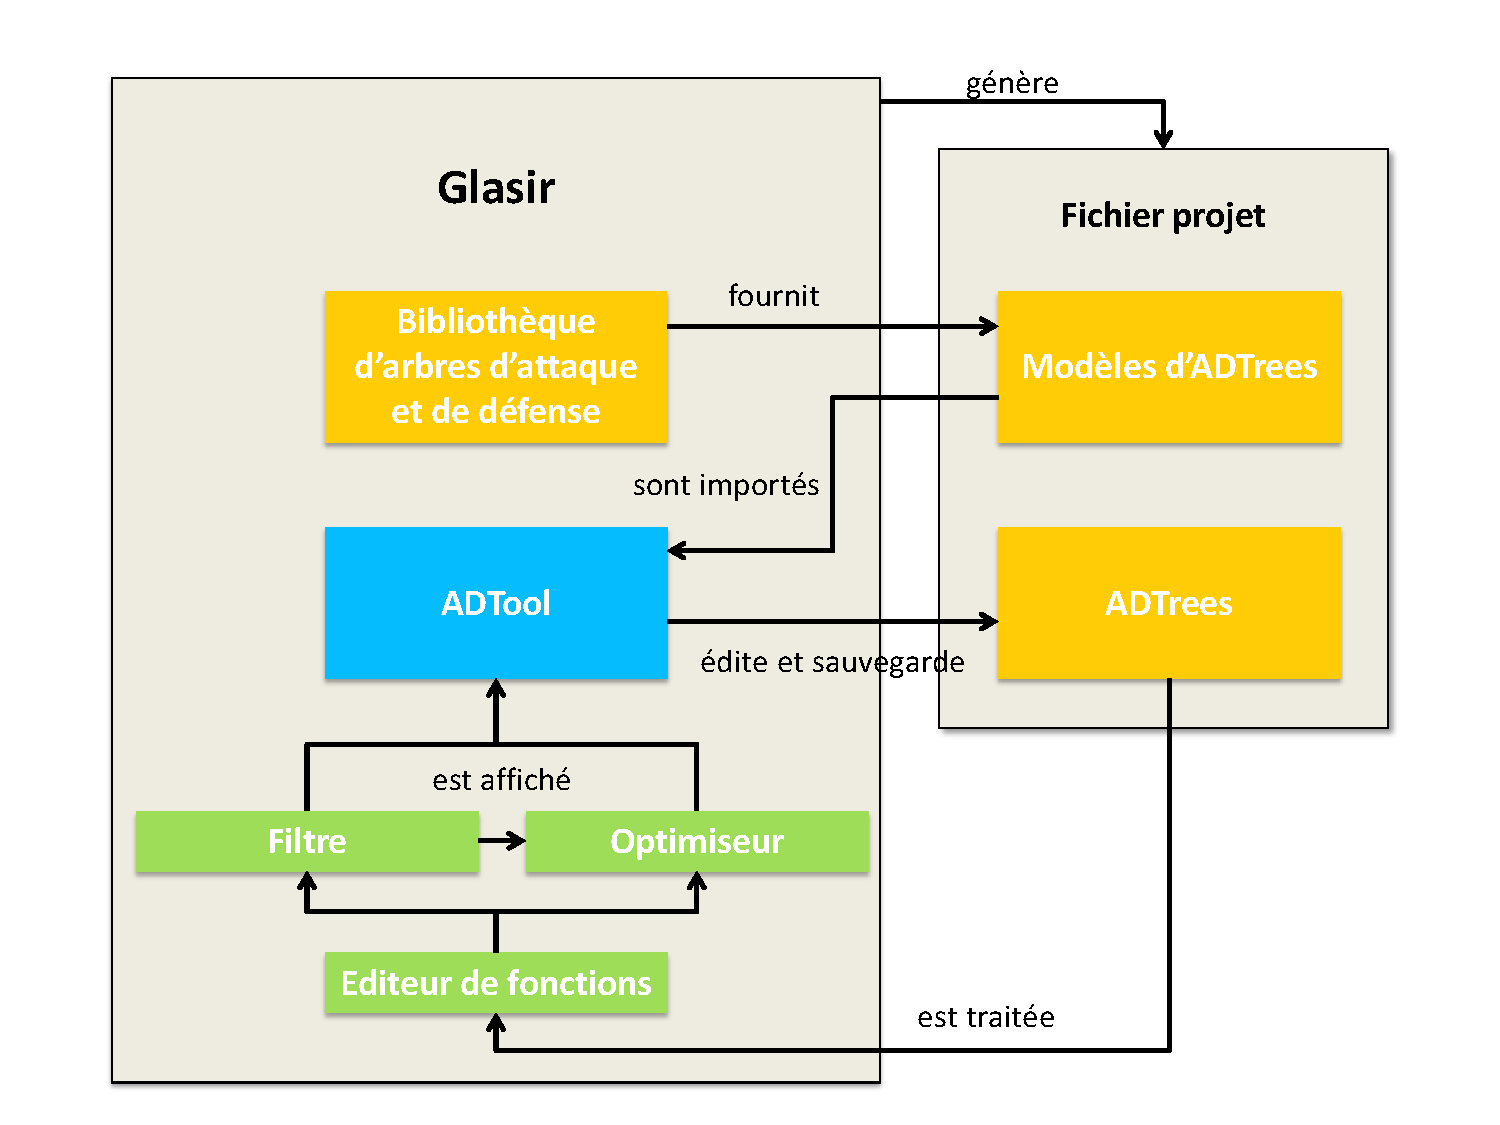
\includegraphics[width=0.8\textwidth]{figure/archiGlasir.pdf}
		\caption{Architecture du logiciel \glasir{}.}
		\label{fig:architecture_Glasir}
	\end{figure}

Comme illustré sur la {\sc Figure} \ref{fig:architecture_Glasir}, \glasir{} est constitué d'une bibliothèque d'ADTrees, d'ADTool et des nouvelles fonctionnalités d'analyse. L'expert réalisant un projet d'analyse à l'aide de \glasir{} utilisera des fichiers projets. Ils contiennent les ADTrees du projet en cours ainsi que les modèles génériques d'ADTrees que l'expert a jugé utiles pour son projet. Ceux-ci proviennent de la bibliothèque d'ADTrees de \glasir{}.
	
Lors de la création d'un projet quelconque, \glasir{} commence par créer le fichier projet correspondant. L'expert va alors créer ou importer ses ADTrees grâce à ADTool. Les modèles de la bibliothèque d'ADTrees utilisés dans le cadre du projet seront également sauvegardés dans le fichier projet, pour gérer leurs éventuelles modifications sans impacter la bibliothèque d'arbres de \glasir{}. L'expert pourra alors définir ses paramètres de synthèse avec l'éditeur de fonction, filtrer grâce au module Filtre ou encore chercher le chemin optimal à l'aide de l'Optimiseur. La prochaine section détaillera l'implémentation de ces modules. 